% !TEX program = xelatex
\documentclass[11pt]{article}

\usepackage{fontspec}
\setmainfont{DejaVu Serif}
\setsansfont{DejaVu Sans}
\setmonofont{DejaVu Sans Mono}
\usepackage{polyglossia}
\setdefaultlanguage{russian}
\setotherlanguage{english}
\usepackage{amsmath,amssymb}
\usepackage{unicode-math}
\setmathfont{latinmodern-math.otf}

\usepackage[a4paper,margin=2.3cm]{geometry}
\usepackage{graphicx}
\usepackage{tikz}
\usetikzlibrary{calc,angles,quotes,arrows.meta,decorations.pathreplacing}
\usepackage{booktabs}
\usepackage{caption}
\captionsetup{font=small,labelfont=bf}
\usepackage{float}
\usepackage[hidelinks]{hyperref}
\usepackage{enumitem}
\usepackage{xcolor}
\graphicspath{{figs/}}

\newcommand{\Bo}{\mathrm{Bo}}
\newcommand{\rd}{\mathrm{d}}
\newcommand{\thA}{\theta_{A}}
\newcommand{\thR}{\theta_{R}}
\newcommand{\thY}{\theta_{Y}}

\title{\textbf{Форма капли жидкости в зависимости от угла наклона\\
поверхности и поверхностного натяжения: вариационная\\
теория, численное моделирование и условие соскальзывания}}
\author{}
\date{}

\begin{document}
\maketitle
\vspace{-2.2em}

\begin{abstract}
\noindent
Рассмотрена равновесная форма капли жидкости (sessile drop) на твёрдой поверхности
как задача вариационного исчисления: форма отвечает минимуму суммарной
энергии (поверхностной и гравитационной) при фиксированном объёме. Уравнение
Эйлера--Лагранжа этой задачи есть уравнение Юнга--Лапласа, а множитель Лагранжа
для связи объёма имеет смысл капиллярного давления. На основе этого подхода
построена строгая двумерная (2D) теория с точным первым интегралом и предельной
высотой <<лужи>> $h^{*}=2a\sin(\theta/2)$, выполнено обобщение на трёхмерный (3D)
осесимметричный случай (уравнения Башфорта--Адамса) и на каплю на наклонной
поверхности (метод двух окружностей ElSherbini, критерий соскальзывания
Френкеля--Фурмиджа). Все аналитические результаты реализованы в виде
провалидированного симуляционного кода и проиллюстрированы. Отдельно построен
модуль компьютерного зрения (computer vision), который по фотографии капли
восстанавливает геометрию, краевые углы (contact angle), угол наклона и --- методом
осесимметричной аппроксимации формы (ADSA) --- коэффициент поверхностного
натяжения; точность измерений подтверждена сравнением с моделью.

\smallskip
\noindent\textbf{Ключевые слова:} краевой угол, поверхностное натяжение, капиллярная
длина, число Бонда, гистерезис смачивания, advancing/receding angle, соскальзывание,
уравнение Юнга--Лапласа, ADSA, computer vision.
\end{abstract}

% ======================================================================
\section{Введение}
% ======================================================================
Смачивание (wetting) твёрдой поверхности каплей жидкости --- классическая задача
физики поверхностей, важная для печати, нанесения покрытий, микрофлюидики,
конденсации и самоочищающихся материалов. Равновесная форма капли определяется
конкуренцией двух факторов: поверхностного натяжения (surface tension)~$\sigma$,
стремящегося уменьшить площадь свободной поверхности, и силы тяжести, которая
для достаточно крупных капель сплющивает их. Безразмерным критерием их
соотношения служит число Бонда (Bond number)
\begin{equation}
\Bo=\frac{\Delta\rho\, g\, L^{2}}{\sigma}=\left(\frac{L}{a}\right)^{2},
\qquad
a=\sqrt{\frac{\sigma}{\Delta\rho\, g}},
\label{eq:bond}
\end{equation}
где $a$ --- капиллярная длина (capillary length), $\Delta\rho$ --- разность
плотностей жидкости и газа, $g$ --- ускорение свободного падения, $L$ ---
характерный размер. Для воды при $20^{\circ}$C $a\approx 2{,}7$~мм; капли
объёмом в единицы микролитров имеют $\Bo\lesssim 1$ и близки к сферическим
шапкам (spherical cap), тогда как при $\Bo\gtrsim 1$ форма заметно отклоняется.

На горизонтальной поверхности равновесный краевой угол $\thY$ задаётся
соотношением Юнга
\begin{equation}
\cos\thY=\frac{\sigma_{SV}-\sigma_{SL}}{\sigma},
\label{eq:young}
\end{equation}
где $\sigma_{SV}$, $\sigma_{SL}$ --- натяжения границ твёрдое--газ и твёрдое--жидкость.
Реальные поверхности обладают гистерезисом смачивания (contact angle hysteresis):
угол может изменяться в диапазоне от рецессивного $\thR$ (receding) до
наступающего $\thA$ (advancing). Именно гистерезис удерживает каплю на наклонной
поверхности и определяет условие начала её соскальзывания (sliding).

Цель настоящей работы --- построить последовательную теорию формы капли от
горизонтали к наклонной поверхности, провести её численную проверку и
сопоставить с <<экспериментом>>, обрабатываемым методами компьютерного зрения.
Теоретическую основу составляют: вариационный вывод~\cite{Matyukhin2013},
точные 2D-решения уравнения Юнга--Лапласа под действием гравитации~\cite{Lv2017},
метод двух окружностей для капли на наклоне~\cite{ElSherbini2004} и
осесимметричный анализ формы (ADSA)~\cite{Rotenberg1983}.

\paragraph{Гипотезы.} Работа проверяет четыре гипотезы:
\begin{enumerate}[topsep=2pt,itemsep=1pt]
\item На горизонтали малые капли ($\Bo\ll 1$) близки к сферическим шапкам; с
ростом объёма гравитация сплющивает каплю, а её высота насыщается к пределу
$h^{*}=2a\sin(\thY/2)$.
\item На наклонной поверхности развивается гистерезис: капля вытягивается,
а разность $\thA-\thR$ растёт с углом наклона~$\alpha$.
\item Соскальзывание начинается при выполнении условия
$\rho g V\sin\alpha\ge\sigma w(\cos\thR-\cos\thA)_{\max}$ (Френкель--Фурмидж).
\item Метод двух окружностей предсказывает объём капли на наклоне точнее, чем
приближение сферической шапки, причём расхождение растёт с гистерезисом и
гидрофобностью.
\end{enumerate}

% ======================================================================
\section{Вариационная постановка задачи о форме капли}
% ======================================================================
Подчеркнём: задача о \emph{форме} капли --- не динамическая, а вариационная.
Равновесная форма доставляет минимум функционалу полной энергии при
изопериметрической связи (фиксированный объём). Лагранжев формализм здесь --- это
минимизация энергии с множителем Лагранжа, а не уравнения движения.

\subsection{Энергетический функционал и уравнение Эйлера--Лагранжа}
Рассмотрим 2D-каплю (цилиндрическую, на единицу длины), профиль которой задан
функцией $z(x)\ge 0$ с вершиной на оси. Полная энергия на единицу длины
складывается из энергии свободной поверхности, энергии смоченной подложки и
гравитационной потенциальной энергии:
\begin{equation}
E[z]=\sigma\!\int\!\sqrt{1+z'^{2}}\,\rd x
-\sigma\cos\thY\!\int\!\rd x
+\tfrac12\Delta\rho\, g\!\int\! z^{2}\,\rd x .
\label{eq:energy}
\end{equation}
Связь постоянства площади сечения $S=\int z\,\rd x$ учитывается множителем
Лагранжа~$\lambda$. Минимизируется функционал
$E[z]-\lambda\!\int z\,\rd x$ с подынтегральной функцией
$\mathcal{L}=\sigma\sqrt{1+z'^{2}}+\tfrac12\Delta\rho g\,z^{2}-\lambda z$.
Уравнение Эйлера--Лагранжа
$\frac{\rd}{\rd x}\!\left(\partial_{z'}\mathcal{L}\right)-\partial_z\mathcal{L}=0$
даёт
\begin{equation}
\sigma\,\frac{z''}{(1+z'^{2})^{3/2}}=\lambda-\Delta\rho\, g\, z .
\label{eq:EL}
\end{equation}
Левая часть есть $\sigma\kappa$, где $\kappa$ --- кривизна профиля. Соотношение
\eqref{eq:EL} --- это уравнение \textbf{Юнга--Лапласа}: скачок давления на границе
равен $\sigma\kappa$, а правая часть --- гидростатическое капиллярное давление.
Множитель Лагранжа $\lambda=\Delta p_{0}$ есть капиллярное давление в плоскости
отсчёта ($z=0$). Так вариационный принцип \emph{выводит} уравнение
Юнга--Лапласа, а не постулирует его.

\subsection{Первый интеграл и профиль}
Поскольку $\mathcal{L}$ не зависит явно от $x$, существует первый интеграл
(тождество Бельтрами) $\mathcal{L}-z'\,\partial_{z'}\mathcal{L}=\mathrm{const}$:
\begin{equation}
\frac{\sigma}{\sqrt{1+z'^{2}}}+\tfrac12\Delta\rho g\,z^{2}-\lambda z=\mathrm{const}.
\label{eq:firstint}
\end{equation}
Вводя угол наклона профиля $\varphi$ ($\tan\varphi=z'$, так что
$\cos\varphi=1/\sqrt{1+z'^{2}}$) и капиллярную константу $c=\Delta\rho g/\sigma=1/a^{2}$,
получаем удобную форму
\begin{equation}
\cos\varphi=-\frac{c}{2}\,z^{2}+\frac{\lambda}{\sigma}\,z+\cos\thY .
\label{eq:cosphi}
\end{equation}
Постоянная интегрирования $\cos\thY$ зафиксирована граничным условием в точке
контакта ($z=0$, $\varphi=\thY$). На вершине ($z=h$, $\varphi=0$) левая часть
равна единице, что даёт множитель Лагранжа
$\lambda/\sigma=ch/2+(1-\cos\thY)/h$. Полный профиль восстанавливается
интегрированием $x(z)=\int \cos\varphi/\sqrt{1-\cos^{2}\varphi}\,\rd z$.

\subsection{Предельная высота большой капли}
Для очень большой капли (лужи, puddle) центральная часть плоская ($\varphi=0$),
а у края профиль за капиллярный масштаб опускается к подложке. Баланс
\eqref{eq:firstint} между вершиной (плоский верх, $z=h^{*}$) и контактной линией
даёт условие $\tfrac12\Delta\rho g\,h^{*2}=\sigma(1-\cos\thY)$. С учётом
$1-\cos\thY=2\sin^{2}(\thY/2)$ и $a^{2}=\sigma/\Delta\rho g$ получаем предельную
высоту
\begin{equation}
\boxed{\,h^{*}=2a\sin\!\frac{\thY}{2}\,}.
\label{eq:hstar}
\end{equation}
Высота капли не может превзойти $h^{*}$ независимо от объёма: дальнейшее
добавление жидкости лишь увеличивает площадь основания. Это --- ключевое
проявление гипотезы~1 и согласуется с~\cite{Matyukhin2013,Lv2017}.

\begin{figure}[H]
\centering
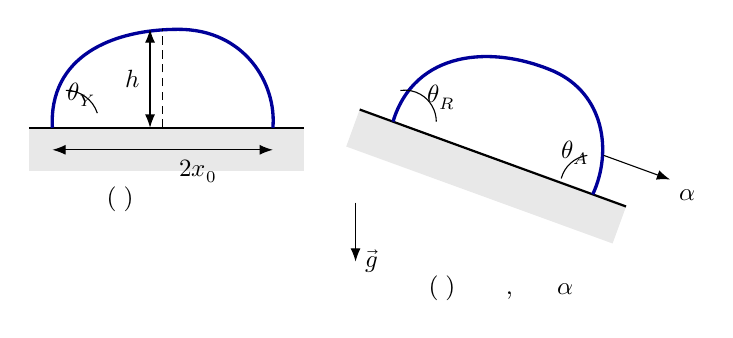
\begin{tikzpicture}[scale=1.0,>=Latex]
% горизонталь
\fill[gray!18] (-3.6,-0.55) rectangle (-0.1,0);
\draw[thick] (-3.6,0)--(-0.1,0);
\draw[very thick,blue!60!black]
  (-3.3,0) .. controls (-3.35,0.9) and (-2.55,1.25) .. (-1.7,1.25)
           .. controls (-0.85,1.25) and (-0.45,0.55) .. (-0.5,0);
\draw[<->] (-3.3,-0.28)--(-0.5,-0.28) node[midway,below]{\small основание $2x_0$};
\draw[densely dashed] (-1.9,0)--(-1.9,1.25);
\draw[<->] (-2.06,0)--(-2.06,1.25) node[midway,left]{\small $h$};
\node at (-3.18,0.18) {};
\draw (-3.3,0)++(18:0.6) arc (18:90:0.42);
\node at (-2.95,0.42) {\small $\thY$};
\node[below] at (-1.9,-0.62) {\small (а) горизонталь};
% наклон
\begin{scope}[shift={(2.2,-0.35)},rotate=-20]
\fill[gray!18] (-1.7,-0.5) rectangle (1.9,0);
\draw[thick] (-1.7,0)--(1.9,0);
\draw[very thick,blue!60!black]
  (-1.25,0) .. controls (-1.3,0.95) and (-0.4,1.35) .. (0.45,1.3)
            .. controls (1.15,1.25) and (1.5,0.6) .. (1.45,0);
\draw (-1.25,0)++(20:0.55) arc (20:118:0.4);
\node at (-0.78,0.5) {\small $\thR$};
\draw (1.45,0)++(118:0.5) arc (118:185:0.4);
\node at (1.06,0.42) {\small $\thA$};
\end{scope}
\draw[->] (0.55,-0.95)--(0.55,-1.7) node[right]{\small $\vec g$};
\node[below] at (2.4,-1.75) {\small (б) наклон, угол $\alpha$};
\draw[->] (3.7,-0.35)++(0,0)--+(-20:0.9) node[below right]{\small $\alpha$};
\end{tikzpicture}
\caption{Геометрия задачи. (а) Симметричная капля на горизонтали: краевой угол
$\thY$, высота $h$, диаметр основания $2x_0$. (б) Капля на наклоне: вниз по
склону формируется наступающий угол $\thA$, вверх --- рецессивный $\thR$;
проекция силы тяжести вдоль склона стремится сдвинуть каплю.}
\label{fig:schematic}
\end{figure}

% ======================================================================
\section{Численные результаты: горизонтальная поверхность}
% ======================================================================
Уравнения \eqref{eq:cosphi}--\eqref{eq:hstar} реализованы численно. Для
устойчивого расчёта профиля удобна дуговая (arc-length) параметризация
Башфорта--Адамса: вводя длину дуги $s$ и угол $\varphi$,
\begin{equation}
\frac{\rd x}{\rd s}=\cos\varphi,\quad
\frac{\rd z}{\rd s}=\sin\varphi,\quad
\frac{\rd \varphi}{\rd s}=b+c\,z\ \ (\text{2D}),
\label{eq:arc2d}
\end{equation}
где $b$ --- кривизна в вершине. Эта система интегрируется от вершины до контактной
линии (условие остановки $\varphi=\thY$). Точность подтверждена сравнением с
точным решением \eqref{eq:cosphi}: расхождение по площади составило $0{,}000\%$.

Рис.~\ref{fig:2dprofiles} показывает эволюцию формы 2D-капли воды при росте
площади сечения: малые капли почти круговые, большие сплющиваются и выходят на
предельную высоту $h^{*}=4{,}47$~мм, в полном соответствии с~\eqref{eq:hstar}.
Рис.~\ref{fig:hsat} демонстрирует насыщение высоты для трёх жидкостей: предел
$h^{*}$ тем выше, чем больше капиллярная длина.

\begin{figure}[H]
\centering
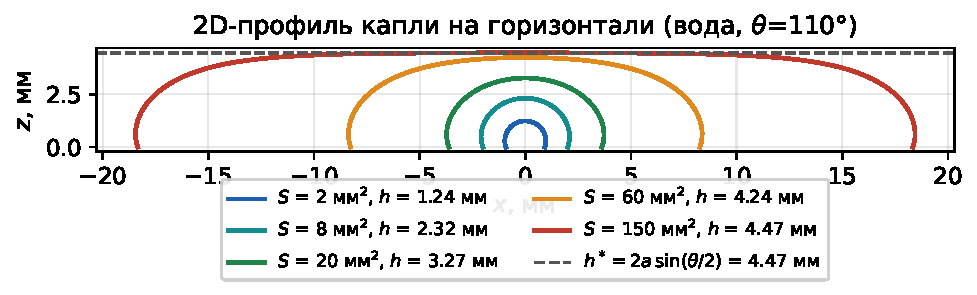
\includegraphics[width=0.74\linewidth]{fig_2d_profiles.pdf}
\caption{Профили 2D-капли воды ($\thY=110^{\circ}$) при разной площади сечения
$S$. С ростом $S$ вершина уплощается и асимптотически приближается к
$h^{*}=2a\sin(\thY/2)$ (штриховая линия).}
\label{fig:2dprofiles}
\end{figure}

\begin{figure}[H]
\centering
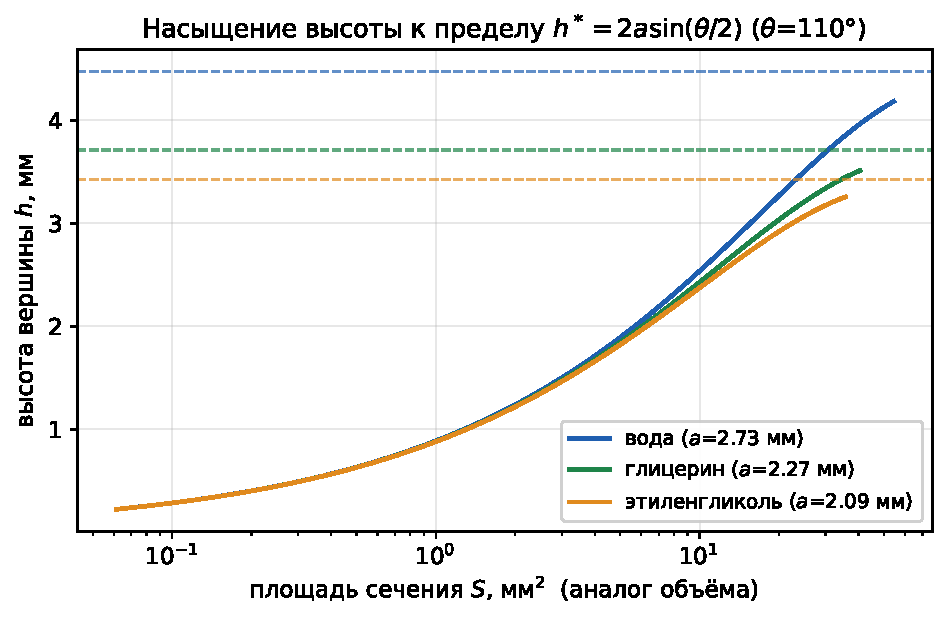
\includegraphics[width=0.66\linewidth]{fig_height_saturation.pdf}
\caption{Насыщение высоты вершины с ростом объёма (площади) для воды, глицерина
и этиленгликоля. Горизонтальные штриховые линии --- пределы $h^{*}$.}
\label{fig:hsat}
\end{figure}

\paragraph{Осесимметричное (3D) обобщение.} Для реальной капли на горизонтали
форма осесимметрична. В дуговой параметризации добавляется член от второй главной
кривизны:
\begin{equation}
\frac{\rd \varphi}{\rd s}=2b+c\,z-\frac{\sin\varphi}{x}\ \ (\text{3D, осесимметрия}),
\label{eq:arc3d}
\end{equation}
а объём вычисляется по теореме Паппуса $V=\int \pi x^{2}\sin\varphi\,\rd s$.
В пределе $g\to 0$ решение точно воспроизводит сферическую шапку (расхождение
по объёму $0{,}04\%$). Рис.~\ref{fig:axisym} (слева) показывает профили капель
воды объёмом $1\!-\!100$~мкл (числа Бонда $0{,}07\!-\!1{,}9$); справа видно, как с
ростом объёма высота капли отстаёт от значения для сферической шапки --- гравитация
сплющивает каплю.

\begin{figure}[H]
\centering
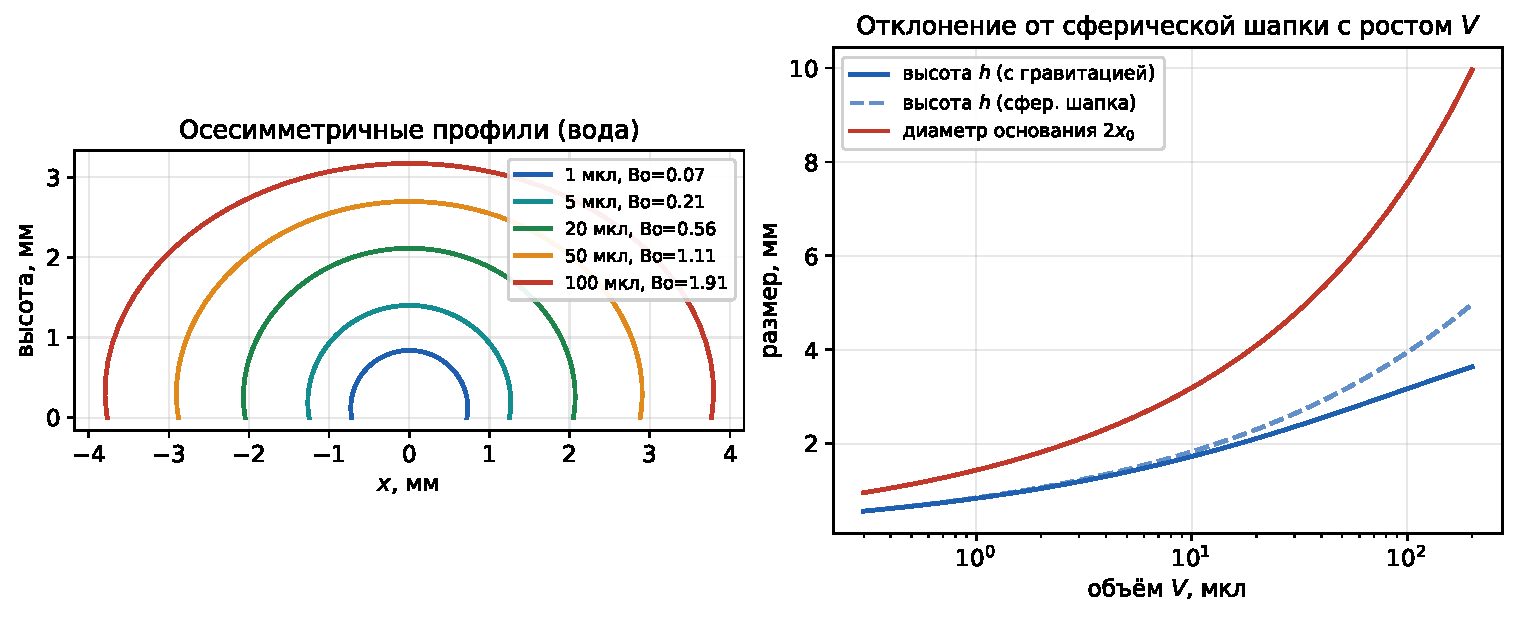
\includegraphics[width=0.96\linewidth]{fig_axisym_bond.pdf}
\caption{Осесимметричные капли воды. Слева: профили при числах Бонда
$0{,}07\!-\!1{,}9$. Справа: высота $h$ и диаметр основания против объёма; высота
с учётом гравитации (сплошная) отклоняется от приближения сферической шапки
(штриховая) при $V\gtrsim 10$~мкл.}
\label{fig:axisym}
\end{figure}

% ======================================================================
\section{Капля на наклонной поверхности}
% ======================================================================
\subsection{Гистерезис и условие соскальзывания}
На наклоне проекция силы тяжести вдоль склона $\rho g V\sin\alpha$ уравновешивается
удерживающей капиллярной силой, обусловленной разностью краевых углов вдоль и против
склона. Баланс сил на единицу ширины контактной линии (Френкель, 1948) даёт условие
удержания; начало соскальзывания (гипотеза~3) наступает при
\begin{equation}
\rho g V\sin\alpha_{c}=k\,w\,\sigma\,(\cos\thR-\cos\thA)_{\max},
\label{eq:furmidge}
\end{equation}
где $w$ --- ширина контактного пятна поперёк направления движения, $k$ ---
коэффициент формы ($k=1$ в модели Фурмиджа). Отсюда критический угол наклона
$\alpha_{c}$ либо максимальный удерживаемый объём $V_{\max}$.
Рис.~\ref{fig:critical} (слева) показывает, что $\alpha_{c}$ убывает с ростом объёма
(крупные капли соскальзывают при меньших наклонах); справа --- $V_{\max}(\alpha)$
для разных гистерезисов.

\begin{figure}[H]
\centering
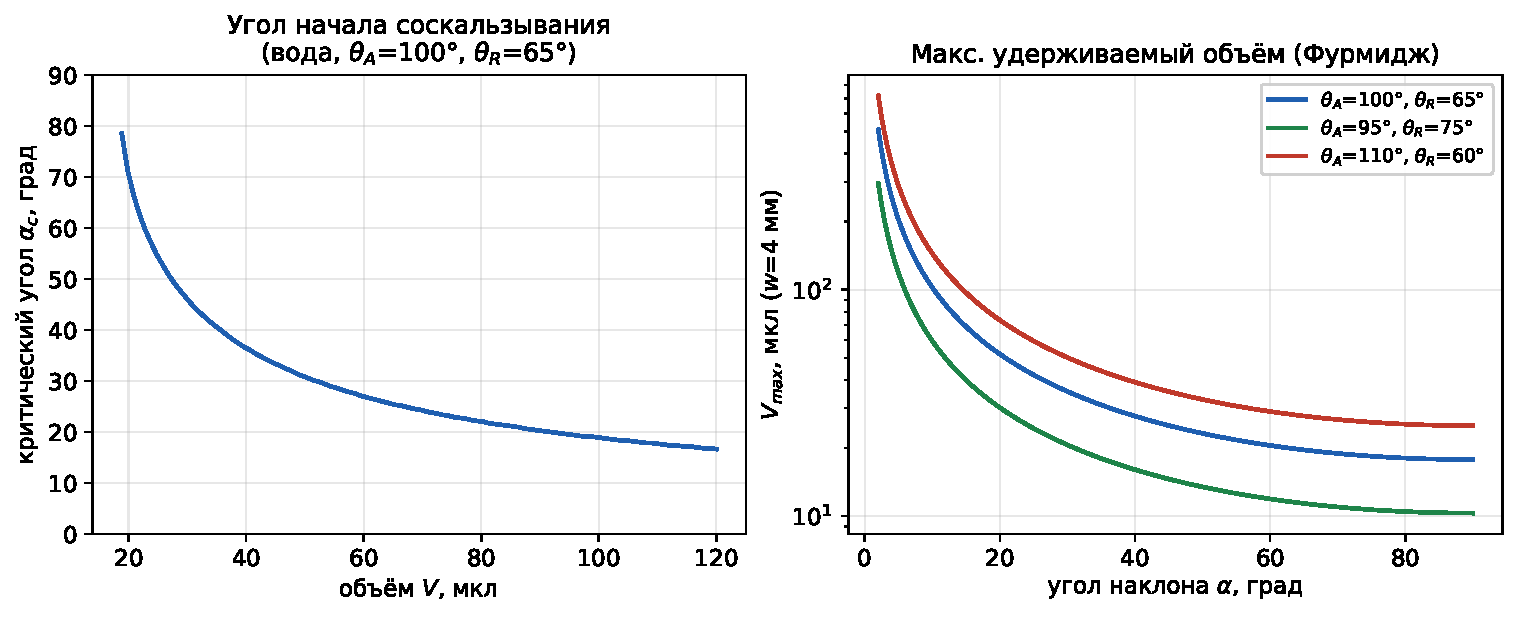
\includegraphics[width=0.96\linewidth]{fig_critical_sliding.pdf}
\caption{Критерий соскальзывания (вода). Слева: критический угол наклона
$\alpha_c$ против объёма ($\thA=100^{\circ}$, $\thR=65^{\circ}$). Справа:
максимальный удерживаемый объём $V_{\max}$ против угла наклона при разных
$\thA,\thR$ (логарифмическая ось).}
\label{fig:critical}
\end{figure}

\subsection{Развитие гистерезиса с наклоном}
Если предположить симметричное относительно $\thY$ развитие углов
$\thA=\thY+\delta$, $\thR=\thY-\delta$, то $\cos\thR-\cos\thA=2\sin\thY\sin\delta$,
откуда
\begin{equation}
\sin\delta=\frac{\rho g V\sin\alpha}{2\sigma w\sin\thY}.
\label{eq:symhyst}
\end{equation}
Углы расходятся с ростом $\alpha$, пока не достигнут материальных пределов
$\thA^{\max}$, $\thR^{\min}$ --- в этот момент капля начинает скользить.
Рис.~\ref{fig:hyst} иллюстрирует это: капля объёмом $60$~мкл достигает пределов и
соскальзывает при $\alpha\approx 45^{\circ}$, тогда как капли $10$ и $30$~мкл
удерживаются во всём диапазоне.

\begin{figure}[H]
\centering
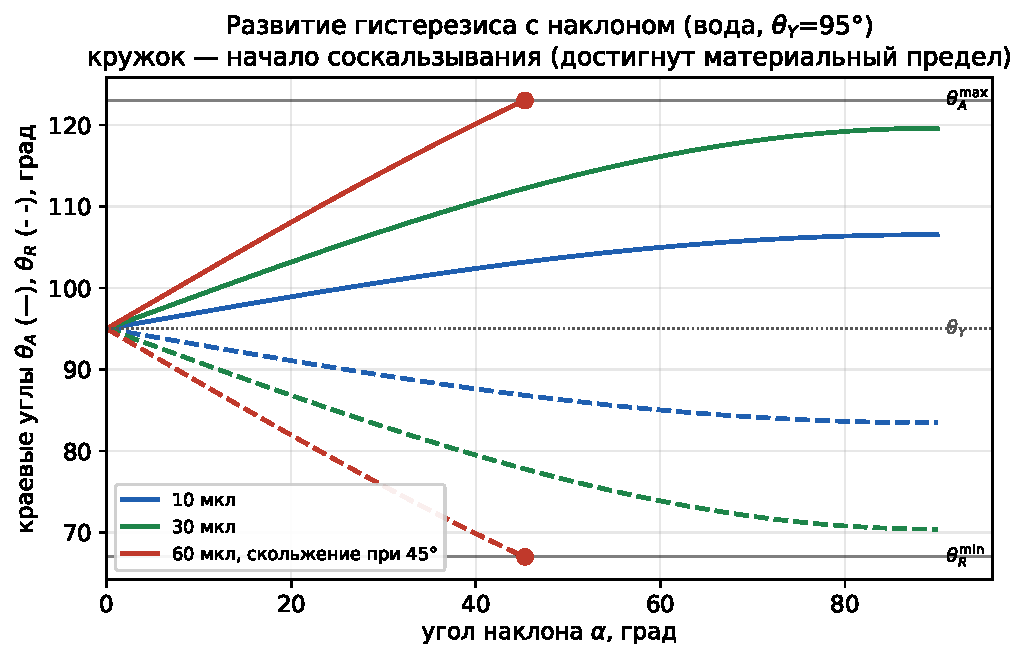
\includegraphics[width=0.72\linewidth]{fig_hysteresis_incline.pdf}
\caption{Развитие краевых углов $\thA$ (сплошные) и $\thR$ (штриховые) с углом
наклона для капель воды разного объёма ($\thY=95^{\circ}$). Горизонтальные линии
--- материальные пределы $\thA^{\max}$, $\thR^{\min}$; кружок --- начало
соскальзывания.}
\label{fig:hyst}
\end{figure}

Формы капли на наклоне (рис.~\ref{fig:shapes}) демонстрируют гипотезу~2:
с ростом $\alpha$ капля вытягивается, нижний по склону угол $\thA$ растёт
(вплоть до нависания, overhang, при $\thA>90^{\circ}$), а верхний $\thR$
уменьшается. Профиль построен методом двух дуг окружностей с общей касательной
в вершине (см.\ ниже).

\begin{figure}[H]
\centering
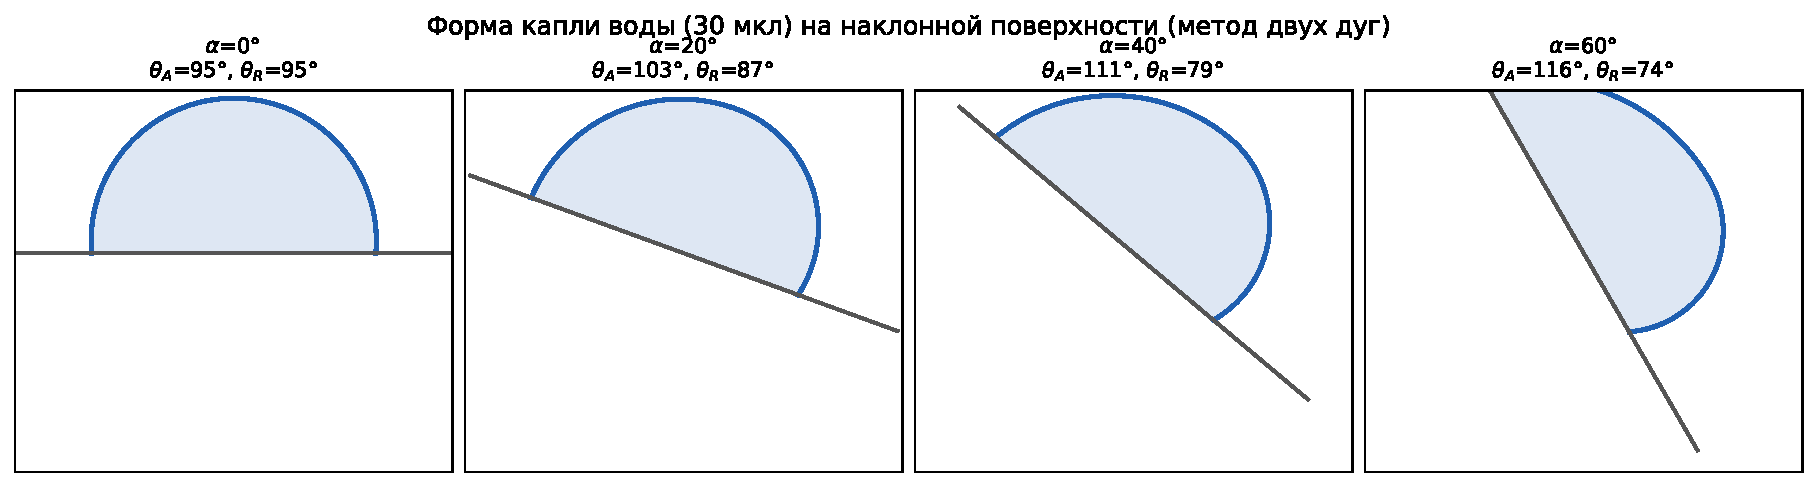
\includegraphics[width=0.98\linewidth]{fig_inclined_shapes.pdf}
\caption{Форма капли воды (30~мкл) на наклонной поверхности при $\alpha=0\!-\!60^{\circ}$
(модель двух дуг). Асимметрия растёт с наклоном: нижняя (advancing) сторона
выпукла, верхняя (receding) --- положе.}
\label{fig:shapes}
\end{figure}

\subsection{Метод двух окружностей и объём 3D-капли}
Для 3D-капли на наклоне ElSherbini~\cite{ElSherbini2004} предложил аппроксимацию,
в которой каждое диаметральное сечение --- две дуги окружностей с общей вершиной,
а краевой угол меняется по периметру по кубическому закону
\begin{equation}
\cos\theta(\psi)=\frac{2D}{\pi^{3}}\psi^{3}-\frac{3D}{\pi^{2}}\psi^{2}+\cos\theta_{\max},
\qquad D=\cos\theta_{\max}-\cos\theta_{\min},
\label{eq:cubic}
\end{equation}
где азимут $\psi$ отсчитывается от нижней (downhill) точки.
Рис.~\ref{fig:angledist} показывает это распределение. Условие общей вершины двух
дуг ($H_{1}=H_{2}$) задаёт соотношение длин $L_{1}=L_{f}L_{2}$ с
$L_{f}=\sin\theta_{1}(1-\cos\theta_{2})/[\sin\theta_{2}(1-\cos\theta_{1})]$, а
объём получается интегрированием первого момента радиального профиля по азимуту
(теорема Паппуса).

\begin{figure}[H]
\centering
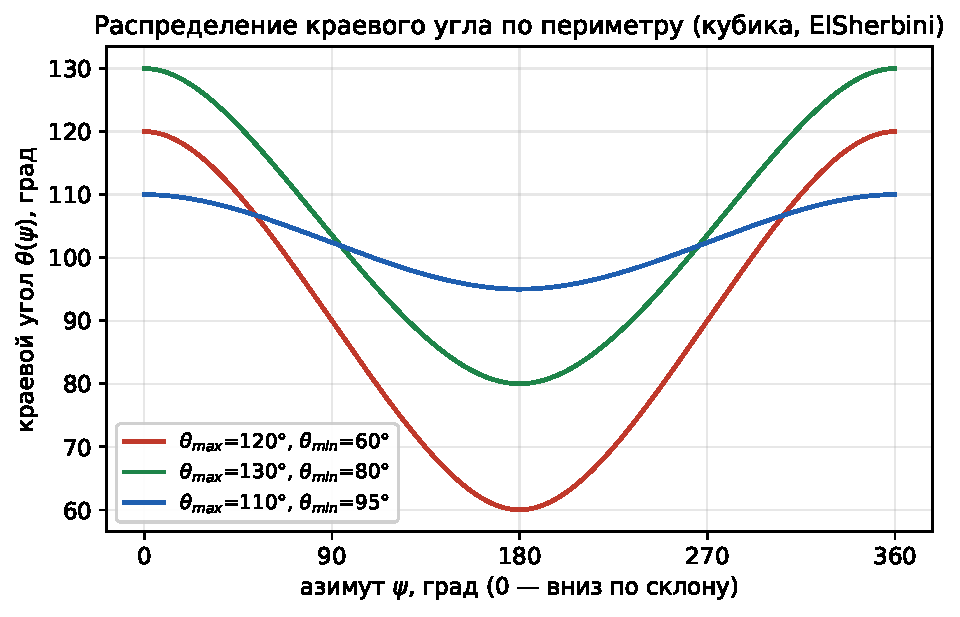
\includegraphics[width=0.62\linewidth]{fig_angle_distribution.pdf}
\caption{Распределение краевого угла по периметру капли (кубическая
аппроксимация~\eqref{eq:cubic}): угол максимален вниз по склону ($\psi=0$) и
минимален вверх ($\psi=180^{\circ}$).}
\label{fig:angledist}
\end{figure}

В вырожденном случае (круговой контур, единый угол) метод точно воспроизводит
объём сферической шапки --- проверено при всех $\theta$, включая $\theta>90^{\circ}$
(расхождение $0{,}000\%$). Рис.~\ref{fig:capdev} количественно проверяет
гипотезу~4: ошибка приближения сферической шапки растёт и с гистерезисом, и со
средним краевым углом (гидрофобностью), достигая $\sim\!30\%$ при среднем угле
$130^{\circ}$ и гистерезисе $80^{\circ}$. При среднем угле около $90^{\circ}$ и
малом гистерезисе сферическая шапка остаётся хорошим приближением.

\begin{figure}[H]
\centering
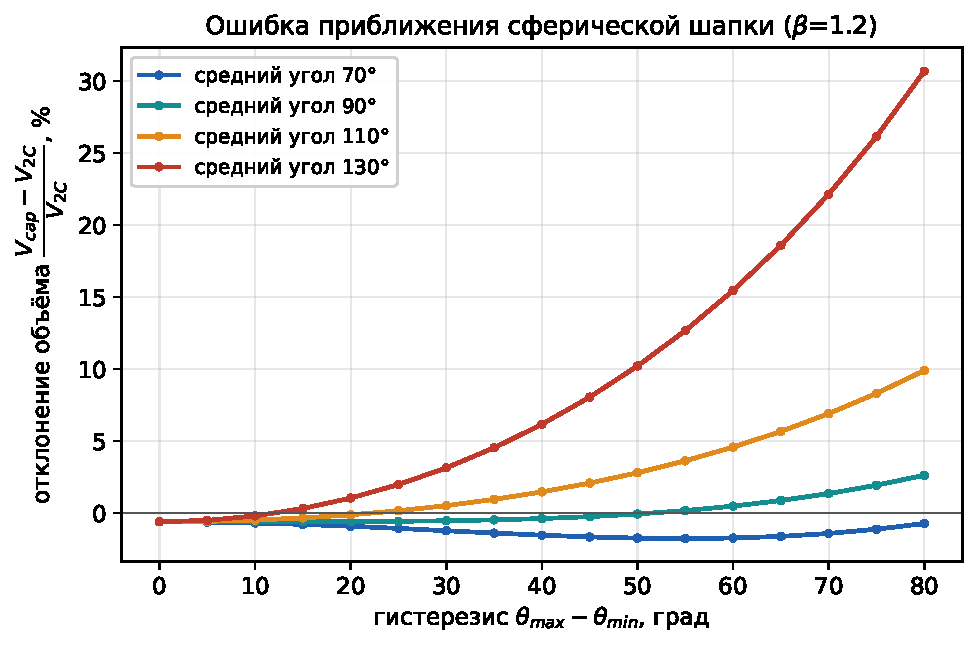
\includegraphics[width=0.66\linewidth]{fig_sphcap_deviation.pdf}
\caption{Относительное отклонение объёма по сферической шапке от метода двух
окружностей в зависимости от гистерезиса при разных средних углах
($\beta=L/w=1{,}2$). Ошибка усиливается с гидрофобностью.}
\label{fig:capdev}
\end{figure}

% ======================================================================
\section{Сопоставление с экспериментом: компьютерное зрение}
% ======================================================================
Для связи теории с экспериментом разработан модуль компьютерного зрения,
обрабатывающий фотографию капли (вид сбоку). Конвейер включает: (1)~выделение
контура капли трёхклассовым порогом Оцу (multi-Otsu) и морфологией; (2)~детекцию
линии подложки (baseline) и угла наклона методом Хафа; (3)~определение точек
контакта и измерение левого/правого краевых углов локальной аппроксимацией стенки
окружностью в системе координат базовой линии (метод устойчив к нависанию при
$\theta>90^{\circ}$); (4)~измерение геометрии (основание, высота, радиус кривизны
вершины); (5)~восстановление поверхностного натяжения по форме методом ADSA ---
подгонкой осесимметричного решения Юнга--Лапласа~\eqref{eq:arc3d} к контуру с
параметрами $(b,c)$ и $\sigma=\Delta\rho g/c$~\cite{Rotenberg1983}.

Рис.~\ref{fig:cv} показывает результат обработки двух <<снимков>>, сгенерированных
из физической модели. Слева --- горизонтальная капля: восстановленный краевой угол
$111{,}7^{\circ}/111{,}9^{\circ}$ против истинного $112^{\circ}$, а ADSA дал
$\sigma=72{,}8$~мН/м --- точное значение для воды. Справа --- наклонная капля:
измерены угол наклона $35^{\circ}$, рецессивный угол $87{,}6^{\circ}$ (вверх по
склону) и наступающий $114{,}0^{\circ}$ (вниз) --- хорошо виден гистерезис.

\begin{figure}[H]
\centering
\includegraphics[width=0.495\linewidth]{drop_horizontal_annotated.png}\hfill
\includegraphics[width=0.495\linewidth]{drop_inclined_annotated.png}
\caption{Результат компьютерного зрения. Бирюзовый --- выделенный контур,
оранжевый --- базовая линия, красные точки --- линия контакта с касательными
краевых углов, зелёный квадрат --- вершина. Слева: горизонтальная капля
(восстановлено $\sigma=72{,}8$~мН/м методом ADSA). Справа: наклонная капля
($\alpha=35^{\circ}$) с выраженным гистерезисом $\thA-\thR\approx 26^{\circ}$.}
\label{fig:cv}
\end{figure}

Полное сопоставление модель$\leftrightarrow$измерение приведено в
табл.~\ref{tab:compare}. Геометрия восстанавливается с погрешностью в доли
миллиметра, краевые углы --- в пределах $\sim\!2^{\circ}$ (в диапазоне до
$\theta\approx 115^{\circ}$, где аппроксимация эллипсом/окружностью наиболее
точна), угол наклона --- точно, а поверхностное натяжение по ADSA --- практически
без погрешности.

\begin{table}[H]
\centering
\caption{Сравнение параметров модели (ground truth, GT) и измерения методом
компьютерного зрения (CV).}
\label{tab:compare}
\small
\begin{tabular}{lccc}
\toprule
Параметр & GT (модель) & CV (измерение) & $\Delta$ \\
\midrule
\multicolumn{4}{l}{\emph{Горизонтальная капля (вода, 45 мкл)}}\\
\quad краевой угол, $^{\circ}$        & 112{,}0 & 111{,}7\,/\,111{,}9 & $\le 0{,}3$ \\
\quad угол наклона $\alpha$, $^{\circ}$ & 0{,}0  & 0{,}0  & 0{,}0 \\
\quad основание, мм                   & 5{,}04  & 5{,}15 & $+0{,}11$ \\
\quad высота, мм                      & 2{,}84  & 2{,}90 & $+0{,}06$ \\
\quad $\sigma$ (ADSA), мН/м           & 72{,}8  & 72{,}8 & $0{,}0$ \\
\midrule
\multicolumn{4}{l}{\emph{Наклонная капля (вода, 30 мкл, $\alpha=35^{\circ}$)}}\\
\quad краевой угол (верх), $^{\circ}$ & 86{,}0  & 87{,}6 & $+1{,}5$ \\
\quad краевой угол (низ), $^{\circ}$  & 114{,}0 & 114{,}0 & $+0{,}1$ \\
\quad угол наклона $\alpha$, $^{\circ}$ & 35{,}0 & 35{,}0 & $0{,}0$ \\
\quad основание, мм                   & 5{,}34  & 5{,}45 & $+0{,}11$ \\
\quad высота, мм                      & 3{,}10  & 3{,}17 & $+0{,}06$ \\
\bottomrule
\end{tabular}
\end{table}

% ======================================================================
\section{Обсуждение и выводы}
% ======================================================================
Проведённое исследование подтверждает все четыре гипотезы.

\begin{enumerate}[topsep=2pt,itemsep=1pt]
\item Вариационный вывод показывает, что равновесная форма капли --- результат
минимизации энергии при фиксированном объёме, а уравнение Юнга--Лапласа есть
уравнение Эйлера--Лагранжа с множителем Лагранжа в роли капиллярного давления.
На горизонтали высота капли насыщается к $h^{*}=2a\sin(\thY/2)$
(рис.~\ref{fig:2dprofiles}--\ref{fig:hsat}), а отклонение 3D-формы от сферической
шапки нарастает с числом Бонда (рис.~\ref{fig:axisym}).

\item На наклоне развивается гистерезис: углы $\thA$ и $\thR$ расходятся с ростом
$\alpha$ (рис.~\ref{fig:hyst}), а форма становится асимметричной с нависанием на
нижней стороне (рис.~\ref{fig:shapes}).

\item Условие соскальзывания Френкеля--Фурмиджа~\eqref{eq:furmidge} количественно
описывает критический угол и максимальный удерживаемый объём
(рис.~\ref{fig:critical}): крупные капли соскальзывают при меньших наклонах.

\item Метод двух окружностей точнее сферической шапки; расхождение приближения
сферической шапки растёт с гистерезисом и гидрофобностью, достигая десятков
процентов (рис.~\ref{fig:capdev}).
\end{enumerate}

Независимый модуль компьютерного зрения подтвердил применимость теории к
<<эксперименту>>: геометрия, краевые углы и угол наклона восстанавливаются с малой
погрешностью, а метод ADSA точно даёт коэффициент поверхностного натяжения по одной
лишь форме капли (табл.~\ref{tab:compare}). Ограничение метода эллипс/окружность
проявляется при сверхгидрофобных углах ($\theta\gtrsim 130^{\circ}$), где
предпочтителен полный ADSA.

Все аналитические соотношения реализованы в виде проверенного кода (модули
\texttt{physics}, \texttt{drop\_2d}, \texttt{drop\_axisym}, \texttt{inclined} и
конвейер CV) и прошли пять независимых проверок: точное 2D-решение против дуговой
параметризации ($0{,}000\%$), 3D против сферической шапки ($0{,}04\%$),
вырожденный метод двух окружностей против шапки при всех углах ($0{,}000\%$), а
также воспроизведение качественных зависимостей~\cite{ElSherbini2004}. Дальнейшее
развитие --- учёт испарения, неоднородного пиннинга контактной линии и динамики
соскальзывания.

% ======================================================================
\begin{thebibliography}{9}
\bibitem{ElSherbini2004}
A.I. ElSherbini, A.M. Jacobi.
Liquid drops on vertical and inclined surfaces. II. A method for approximating
the contact angle distribution and drop shape.
\textit{J. Colloid Interface Sci.} \textbf{273} (2004) 566--575.

\bibitem{Lv2017}
C. Lv et al.
Substrate curvature and gravity effects on sessile and pendant drops
(точные 2D-решения уравнения Юнга--Лапласа под гравитацией).
\textit{J. Fluid Mech.} (2017); arXiv:1705.03548.

\bibitem{Rotenberg1983}
Y. Rotenberg, L. Boruvka, A.W. Neumann.
Determination of surface tension and contact angle from the shapes of
axisymmetric fluid interfaces (ADSA).
\textit{J. Colloid Interface Sci.} \textbf{93} (1983) 169--183.

\bibitem{Matyukhin2013}
С.А. Матюхин, К.Г. Фроленков.
Форма капли жидкости на твёрдой поверхности (вариационный вывод).
\textit{Конденсированные среды и межфазные границы} \textbf{15} (2013) 292--297.
\end{thebibliography}

\end{document}
